\chapter{Results}

This chapter will present the partial results we obtained in this project. First, we will present the different technologies we used in producing droplets and how we overcame arising technical challenges. Then we introduce how we identified an antibiotic producer and its respective target using halo assays to conduct a library screening. Lastly we focus on biological problems which arose due to the unique nature of the droplet environment and issues with the chosen antibiotic production strain in general. 

\section{Successful droplet production}
\begin{figure}
\centering
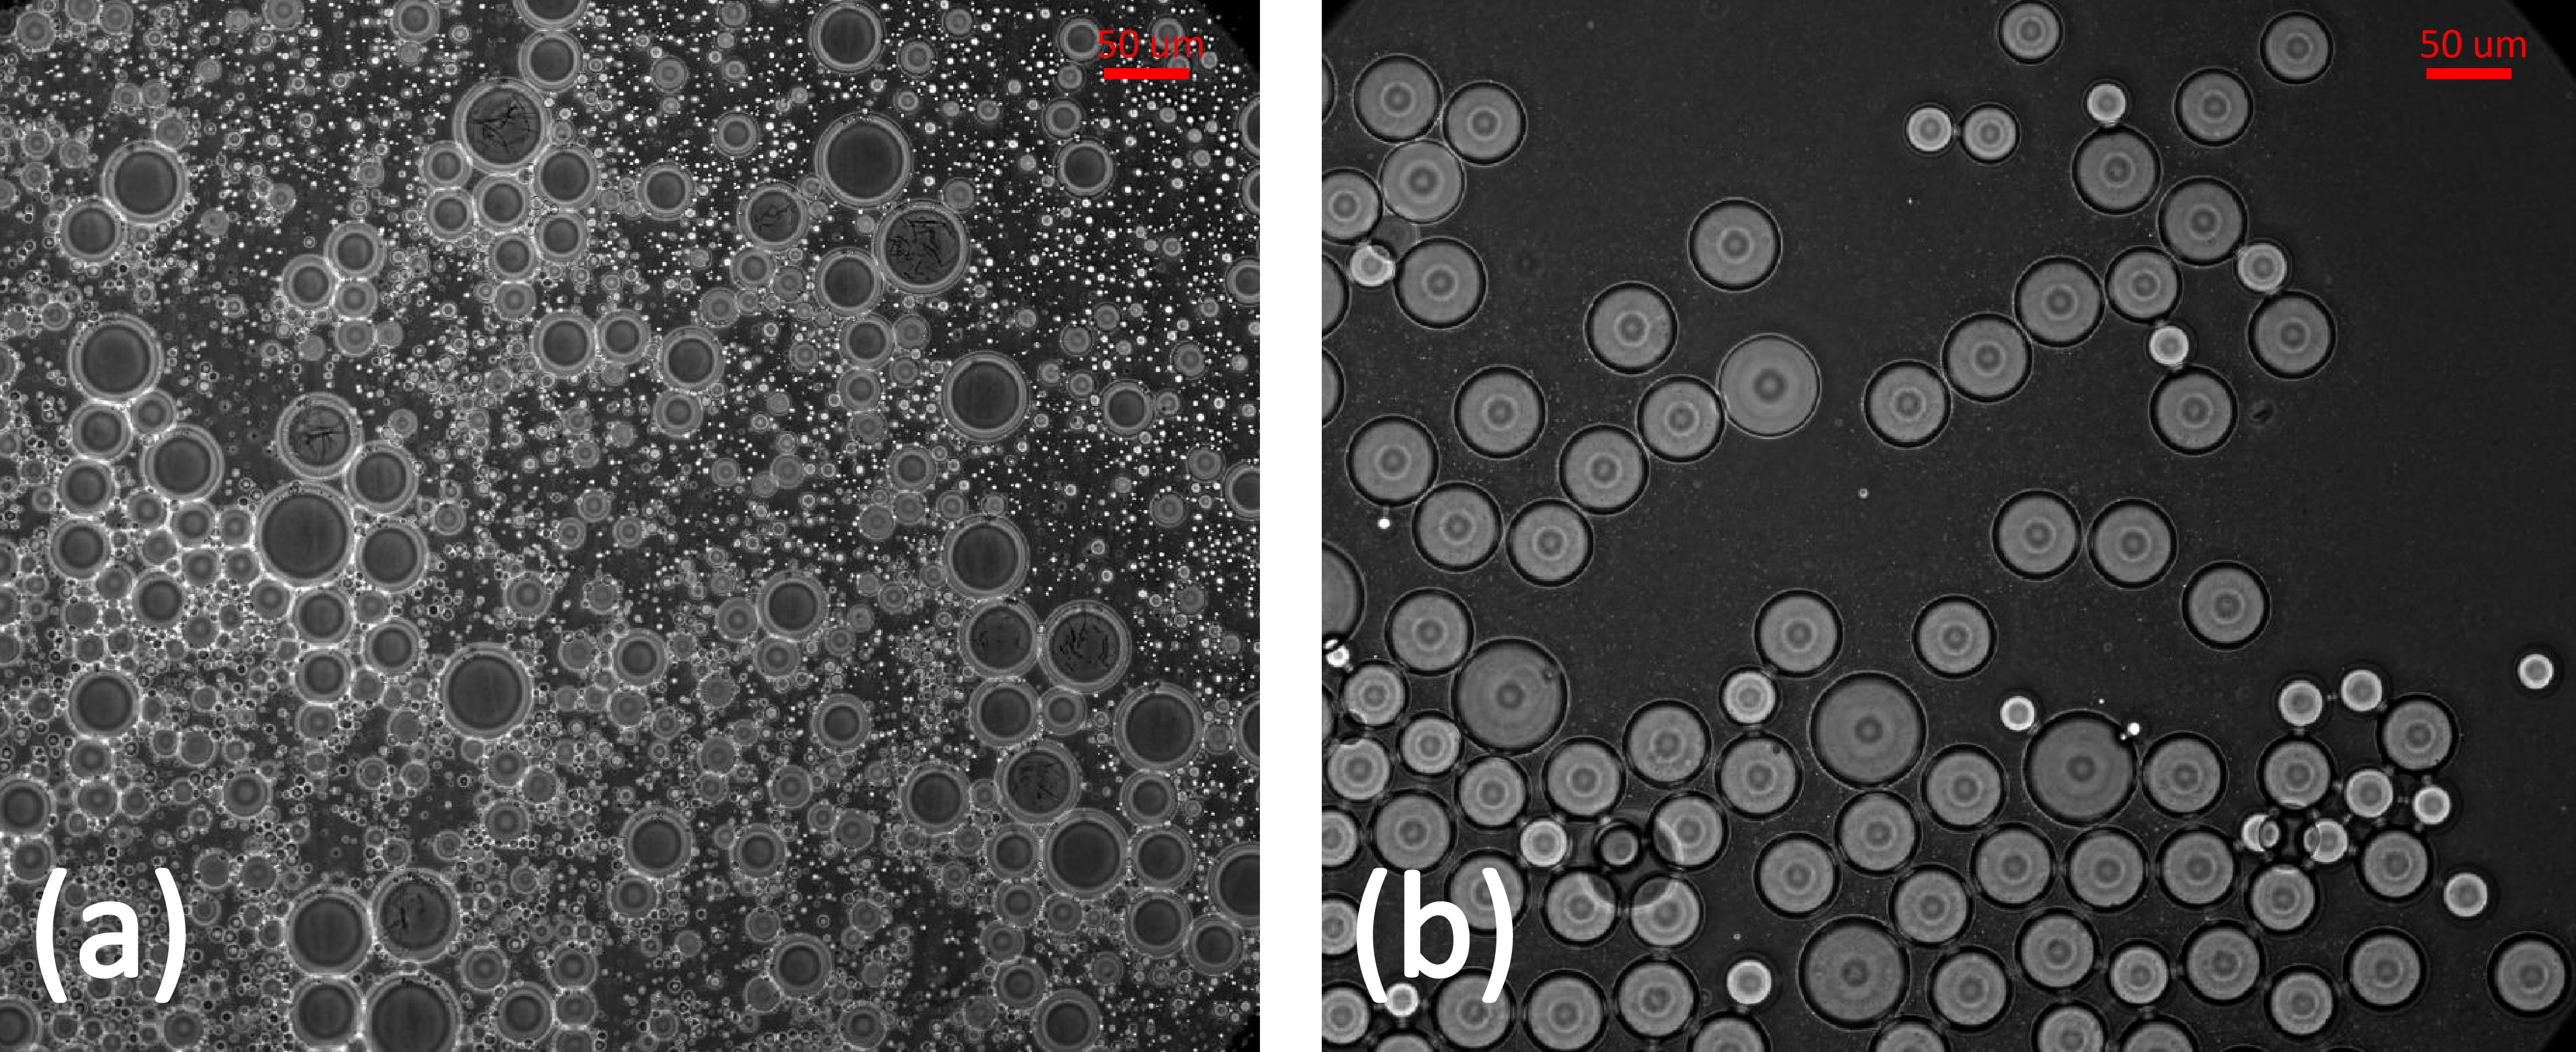
\includegraphics[width=\linewidth]{graphics/2025_09_30_droplets_fig5.png}
\caption{\textbf{Comparison of bulk droplets and on-chip droplets reveals broad size distribution in bulk droplets} In (a) we see bulk microdroplets after 21h of incubation (30$^\circ$C) without shaking. A broad distribution of droplet sizes can be observed. In bigger droplets, bacteria are observed. In (b), we see on-chip microdroplets. These are more uniform in size, especially a lower size limit can be observed and the bigger droplets are probably merged single droplets.}
\label{fig:results_droplet_bulk_vs_chip}
\end{figure}
We employed both methods, previously described, to produce droplets succesfully.~Figure~\ref{fig:results_droplet_bulk_vs_chip} shows the resulting droplets from employing both methods. When using magnetic stirrers to create bulk droplets, we obtain stable microdroplets which are stable even over longer periods of time and incubation. The size distribution is very broad and the upper limit allows significant bacterial growth in droplets. In contrast to this method, when using aa commercially available microfluidic chip, we can produce droplets with a very narrow size distribution. These droplets also allow for bacterial growth but producing the droplets is more challenging due to sensitivity of pressures and possible accumulation of debris in the chip which can block production. Nevertheless, for our pilot experiments we use the microfluidic chip to improve reproducibility of droplets and experiments.

\section{Recommended oil evaporates rapidly}
\begin{figure}
\centering
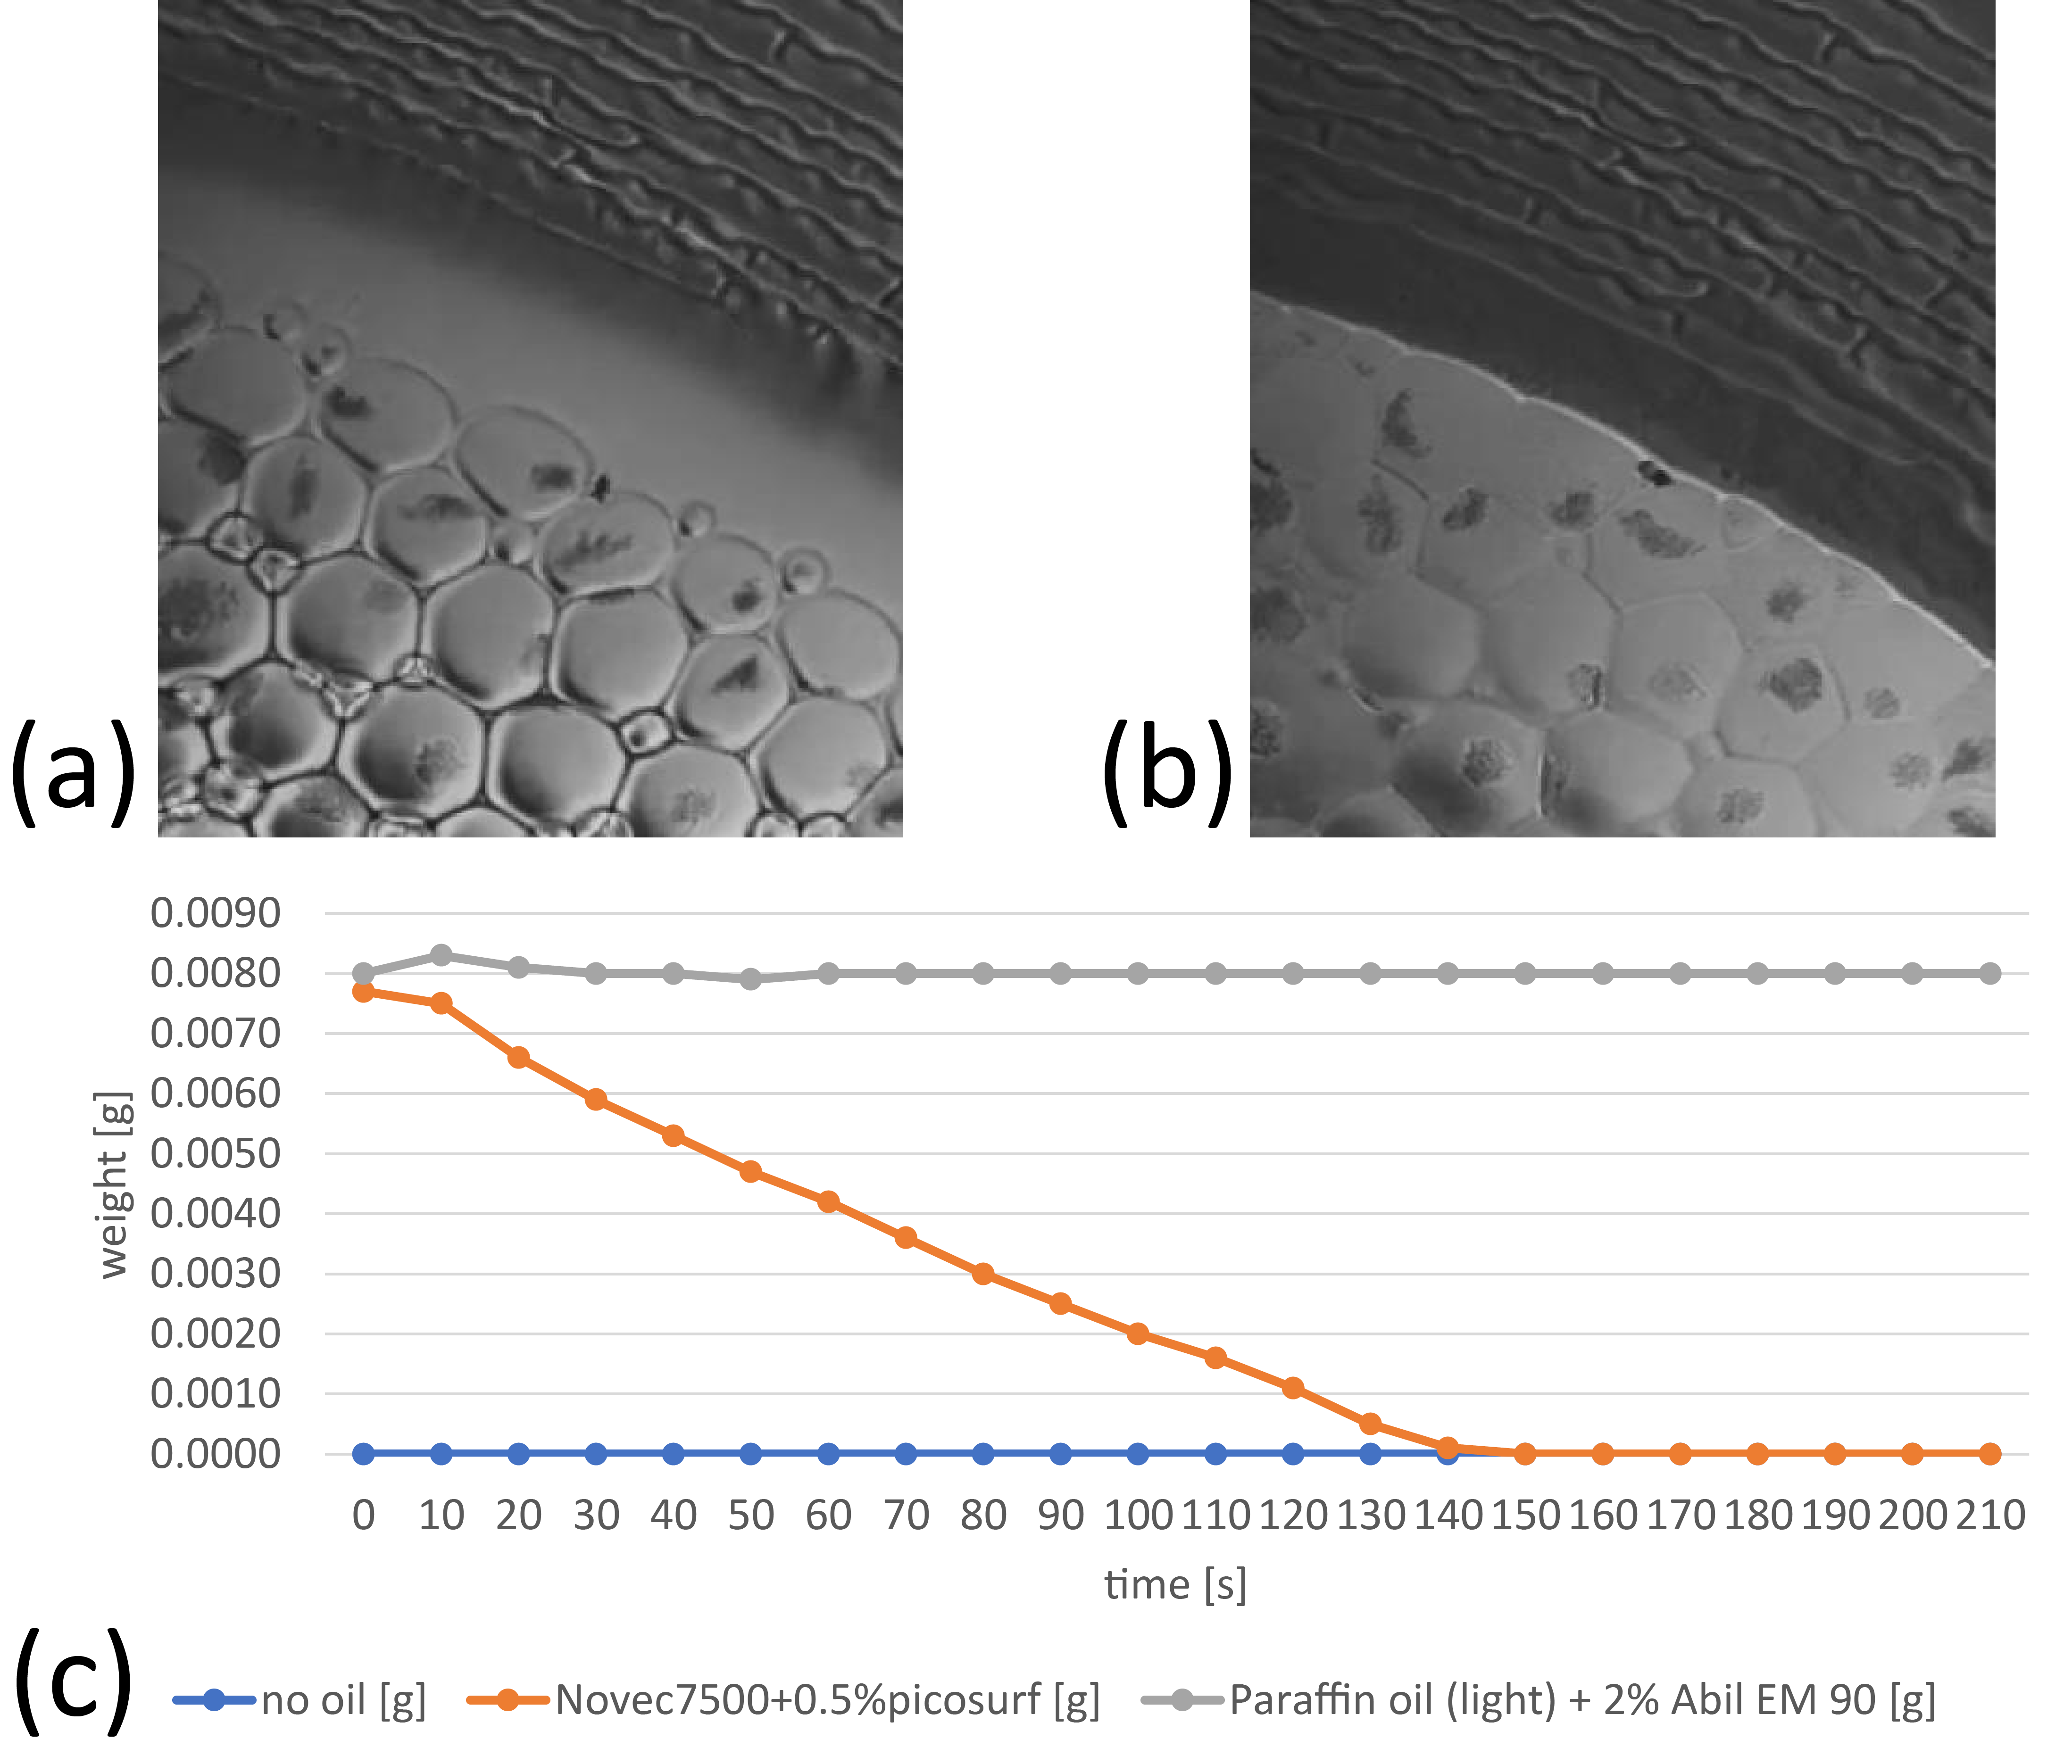
\includegraphics[width=\linewidth]{graphics/2025_09_30_droplets_fig6.png}
\caption{\textbf{Novec\textsuperscript{TM}7500 rapidly evaporates and does not allow for droplet incubation and observation} Using a recommended oil for the commercial microfluidic chip we used, we observed an odd phenomenon. Upon inspection under the microscope we observed a wave-like pattern (a) which led to the droplets coming under tension and finally merge (b). Further investigation and a small control, where we added small amounts of Novec\textsuperscript{TM}7500 oil on a glass slide in a scale revealed continuous, rapid evaporation while Paraffin oil does not evaporate (d).}
\label{fig:results_oil_evaporation}
\end{figure}
While we were able to produce stable, observable droplets using Paraffin oil, we did not succeed to observe stable droplets using Novec\textsuperscript{TM}7500 which was recommended by the manufacturer of our microfluidic chip. Interestingly, we were able to produce droplets and incubate them over long time. However, upon exposure to air, the oil exhibited wave dynamics when observed under a microscope (Figure~\ref{fig:results_oil_evaporation}a) and after a short time, the droplets got pushed together and finally surface tension led to collapse and merging of the distinct droplet environments (Figure~\ref{fig:results_oil_evaporation}b). This led us to suspect that the oil might evaporate in our conditions and indeed, when using a glass slide on a high-precision scale and adding a $5 \mu l$ drop of oil, we observe a rapid weight loss, indicating evaporation. For Paraffin oil, which we also use to create droplets, we do not observe this phenomenon. Therefore, we focused on producing droplets solely with Paraffin oil (Figure~\ref{fig:results_oil_evaporation}c).

\section{Identifying producer-target pair}
\begin{figure}
\centering
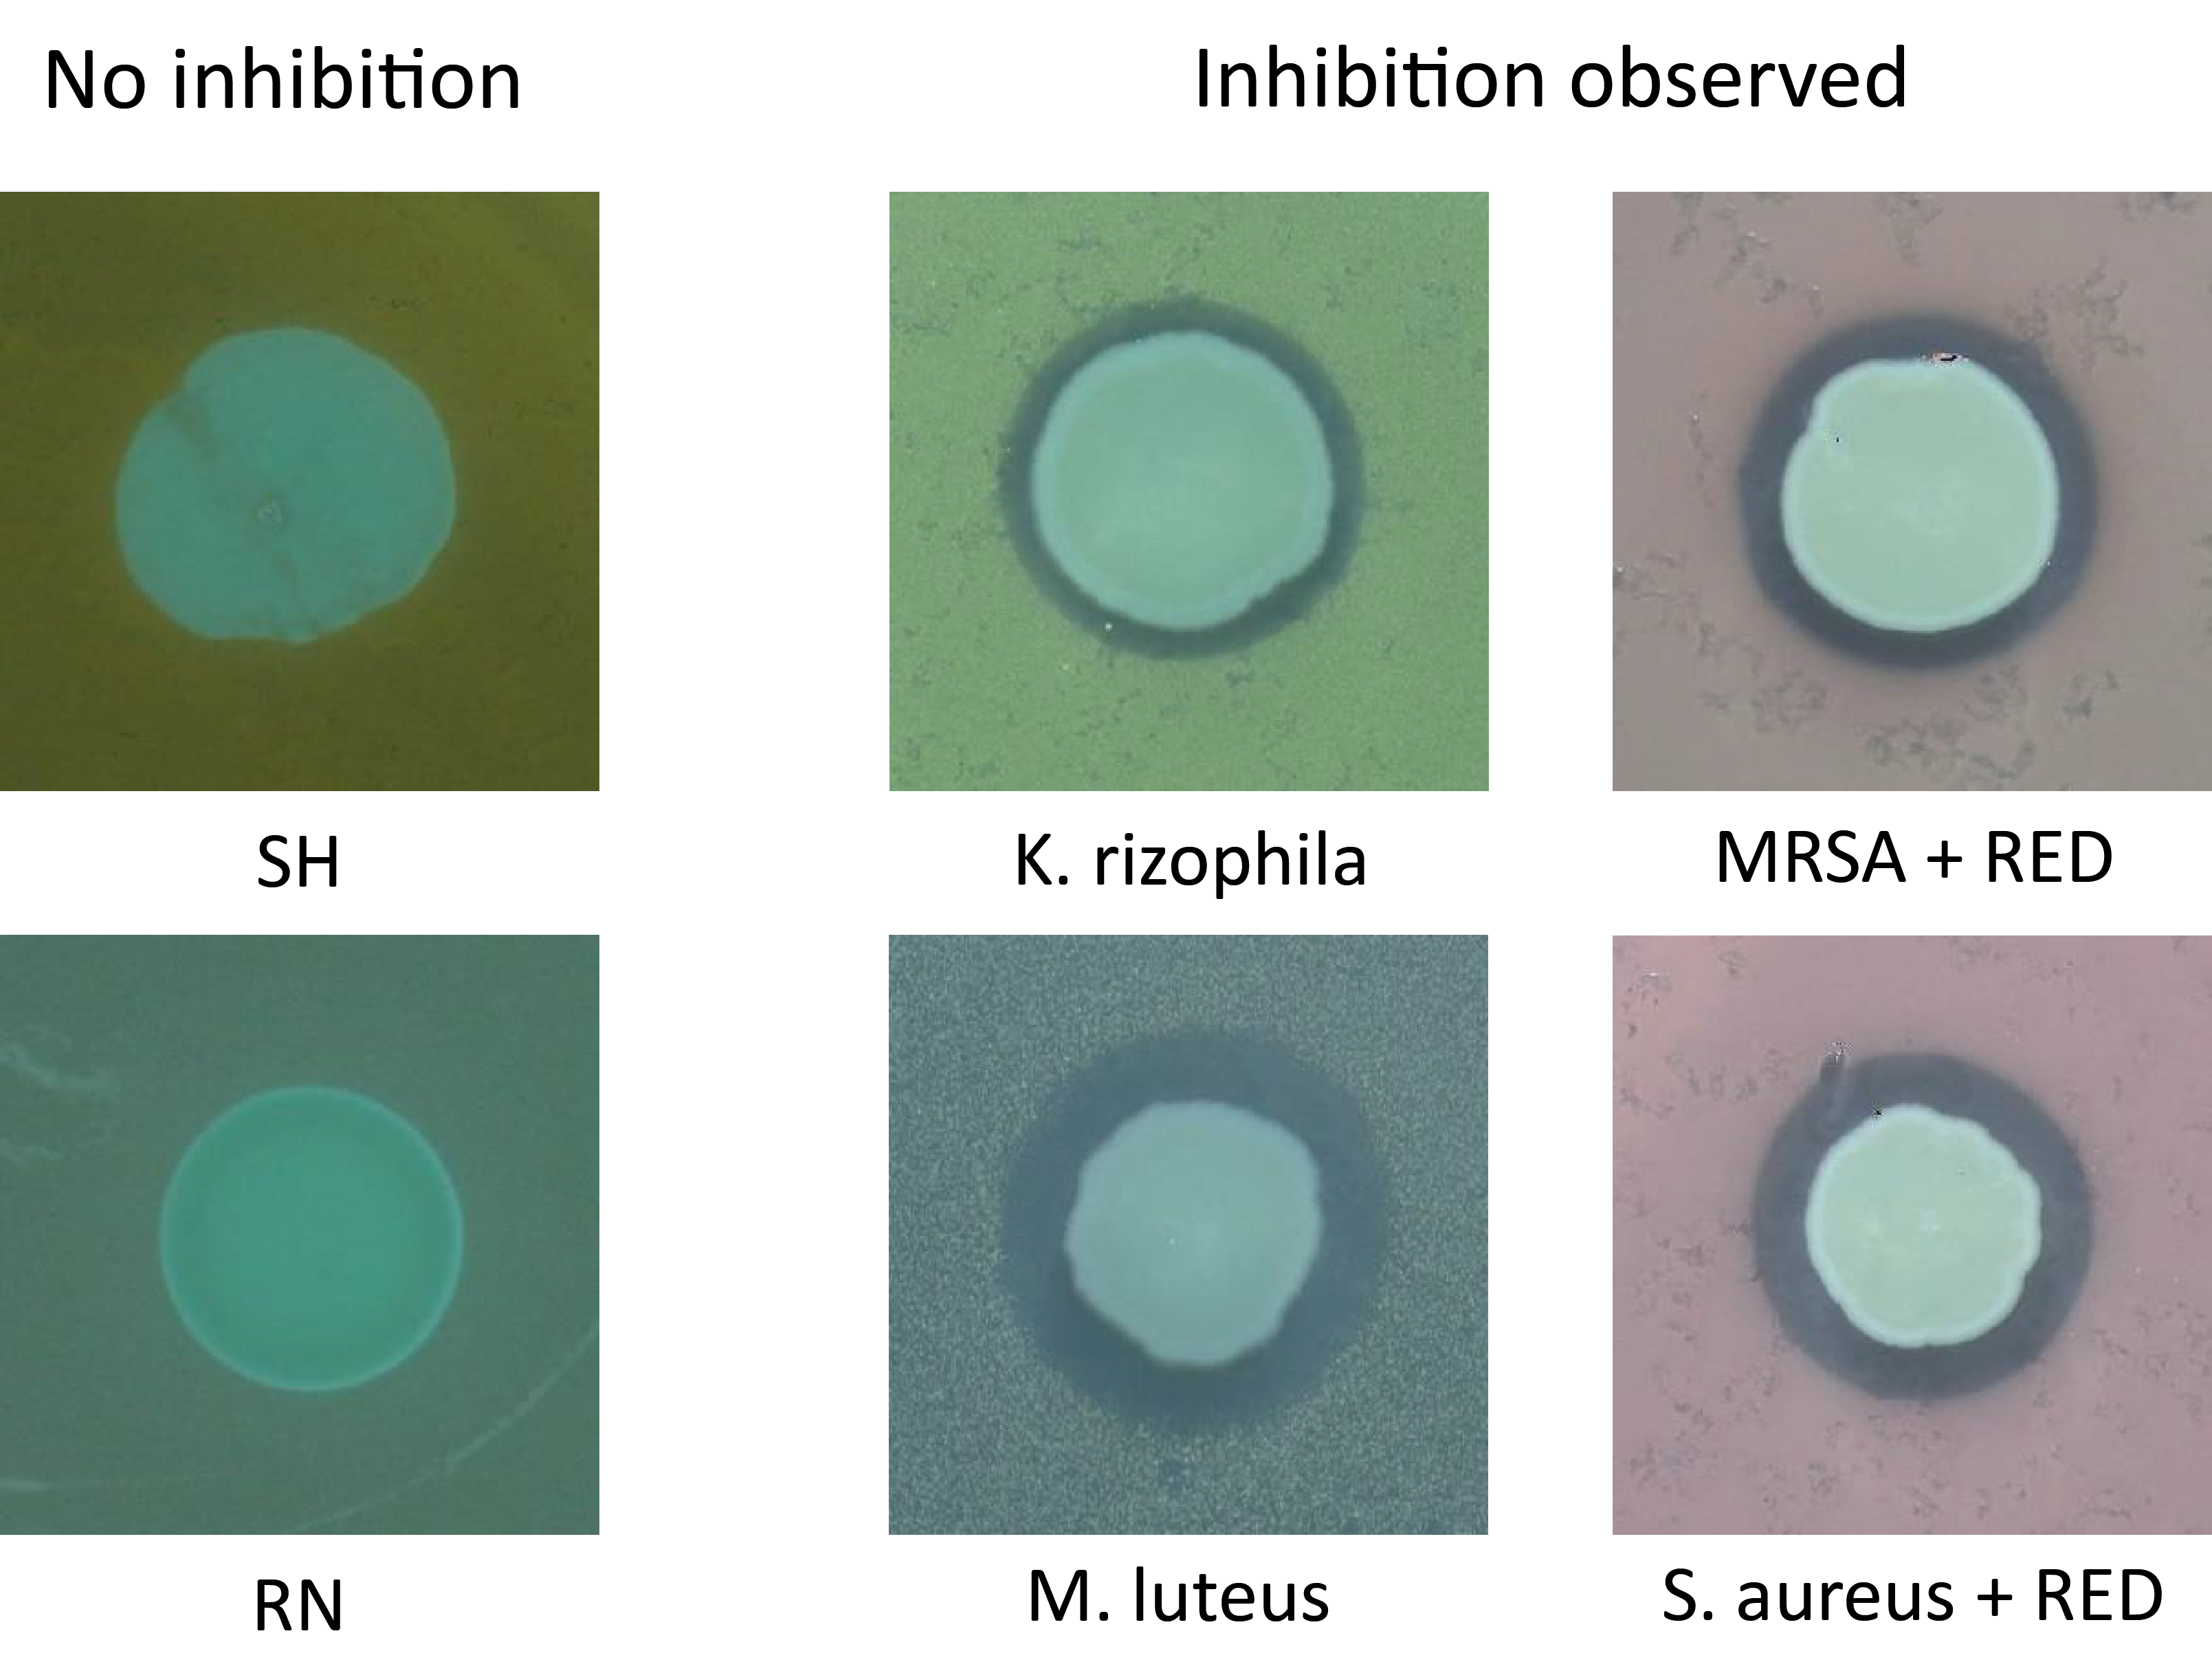
\includegraphics[width=\linewidth]{graphics/2025_09_30_droplets_fig7.png}
\caption{\textbf{Halo assay for library of target strains identifies \textit{S. aureus} as potential target} Using halo assays, we conducted a broad screening of very distinct bacterial strains to determine possible target strains for the chosen \textit{Bacillus subtilis} producer strain. Some natural isolates from our collection showed no inhibition but we observed several strains which exhibit inhibition. Among them the commonly used susceptibility test strain of \textit{Koccuria rizophila} but also clinically relevant strains of \textit{Staphyloccous aureus}, both methycillin-resistant (MRSA) and sensitive.}
\label{fig:results_sensitive_screening}
\end{figure}
Previous research in our lab~\cite{Gerardin2016-ac} used a colicin-producing \textit{E. coli} strain as an antibiotic producing strain. This is less feasible in droplets due to the inherent nature of colicin. In order for bacteria to release colicin, these bacteria need to lyse. As the volume in droplets is very limited, we inoculate the droplets with low numbers of bacteria. The need of lysis therefore does not allow to use colicin in our setup.
Instead we focused on other antibiotics, based on several criteria like culturability in growth media also suitable for possible target strains, small molecule antibiotic, to allow for beneficial mutations and hydrophilicity to avoid diffusion outside of the droplets. Based on these criteria, we chose a subtilin-producing \textit{B. subtilis} strain~\cite{Stein2002-nv, Zhang2022-ee} as the antibiotic producing strain.
After choosing our antibiotic producing strain, we used the well established halo-assay method to screen a collection of possible target strains, selected based on similar growth rate and easy culture conditions. We observe inhibition for several of the possible targets~(Figure~\ref{fig:results_sensitive_screening}). Based on these results, we chose a \textit{Staphylococcus aureus} strain due to the large inhibition zone combined with its clinical significance. We ...

\section{B. subtilis stressed in droplets}
\begin{figure}
\centering
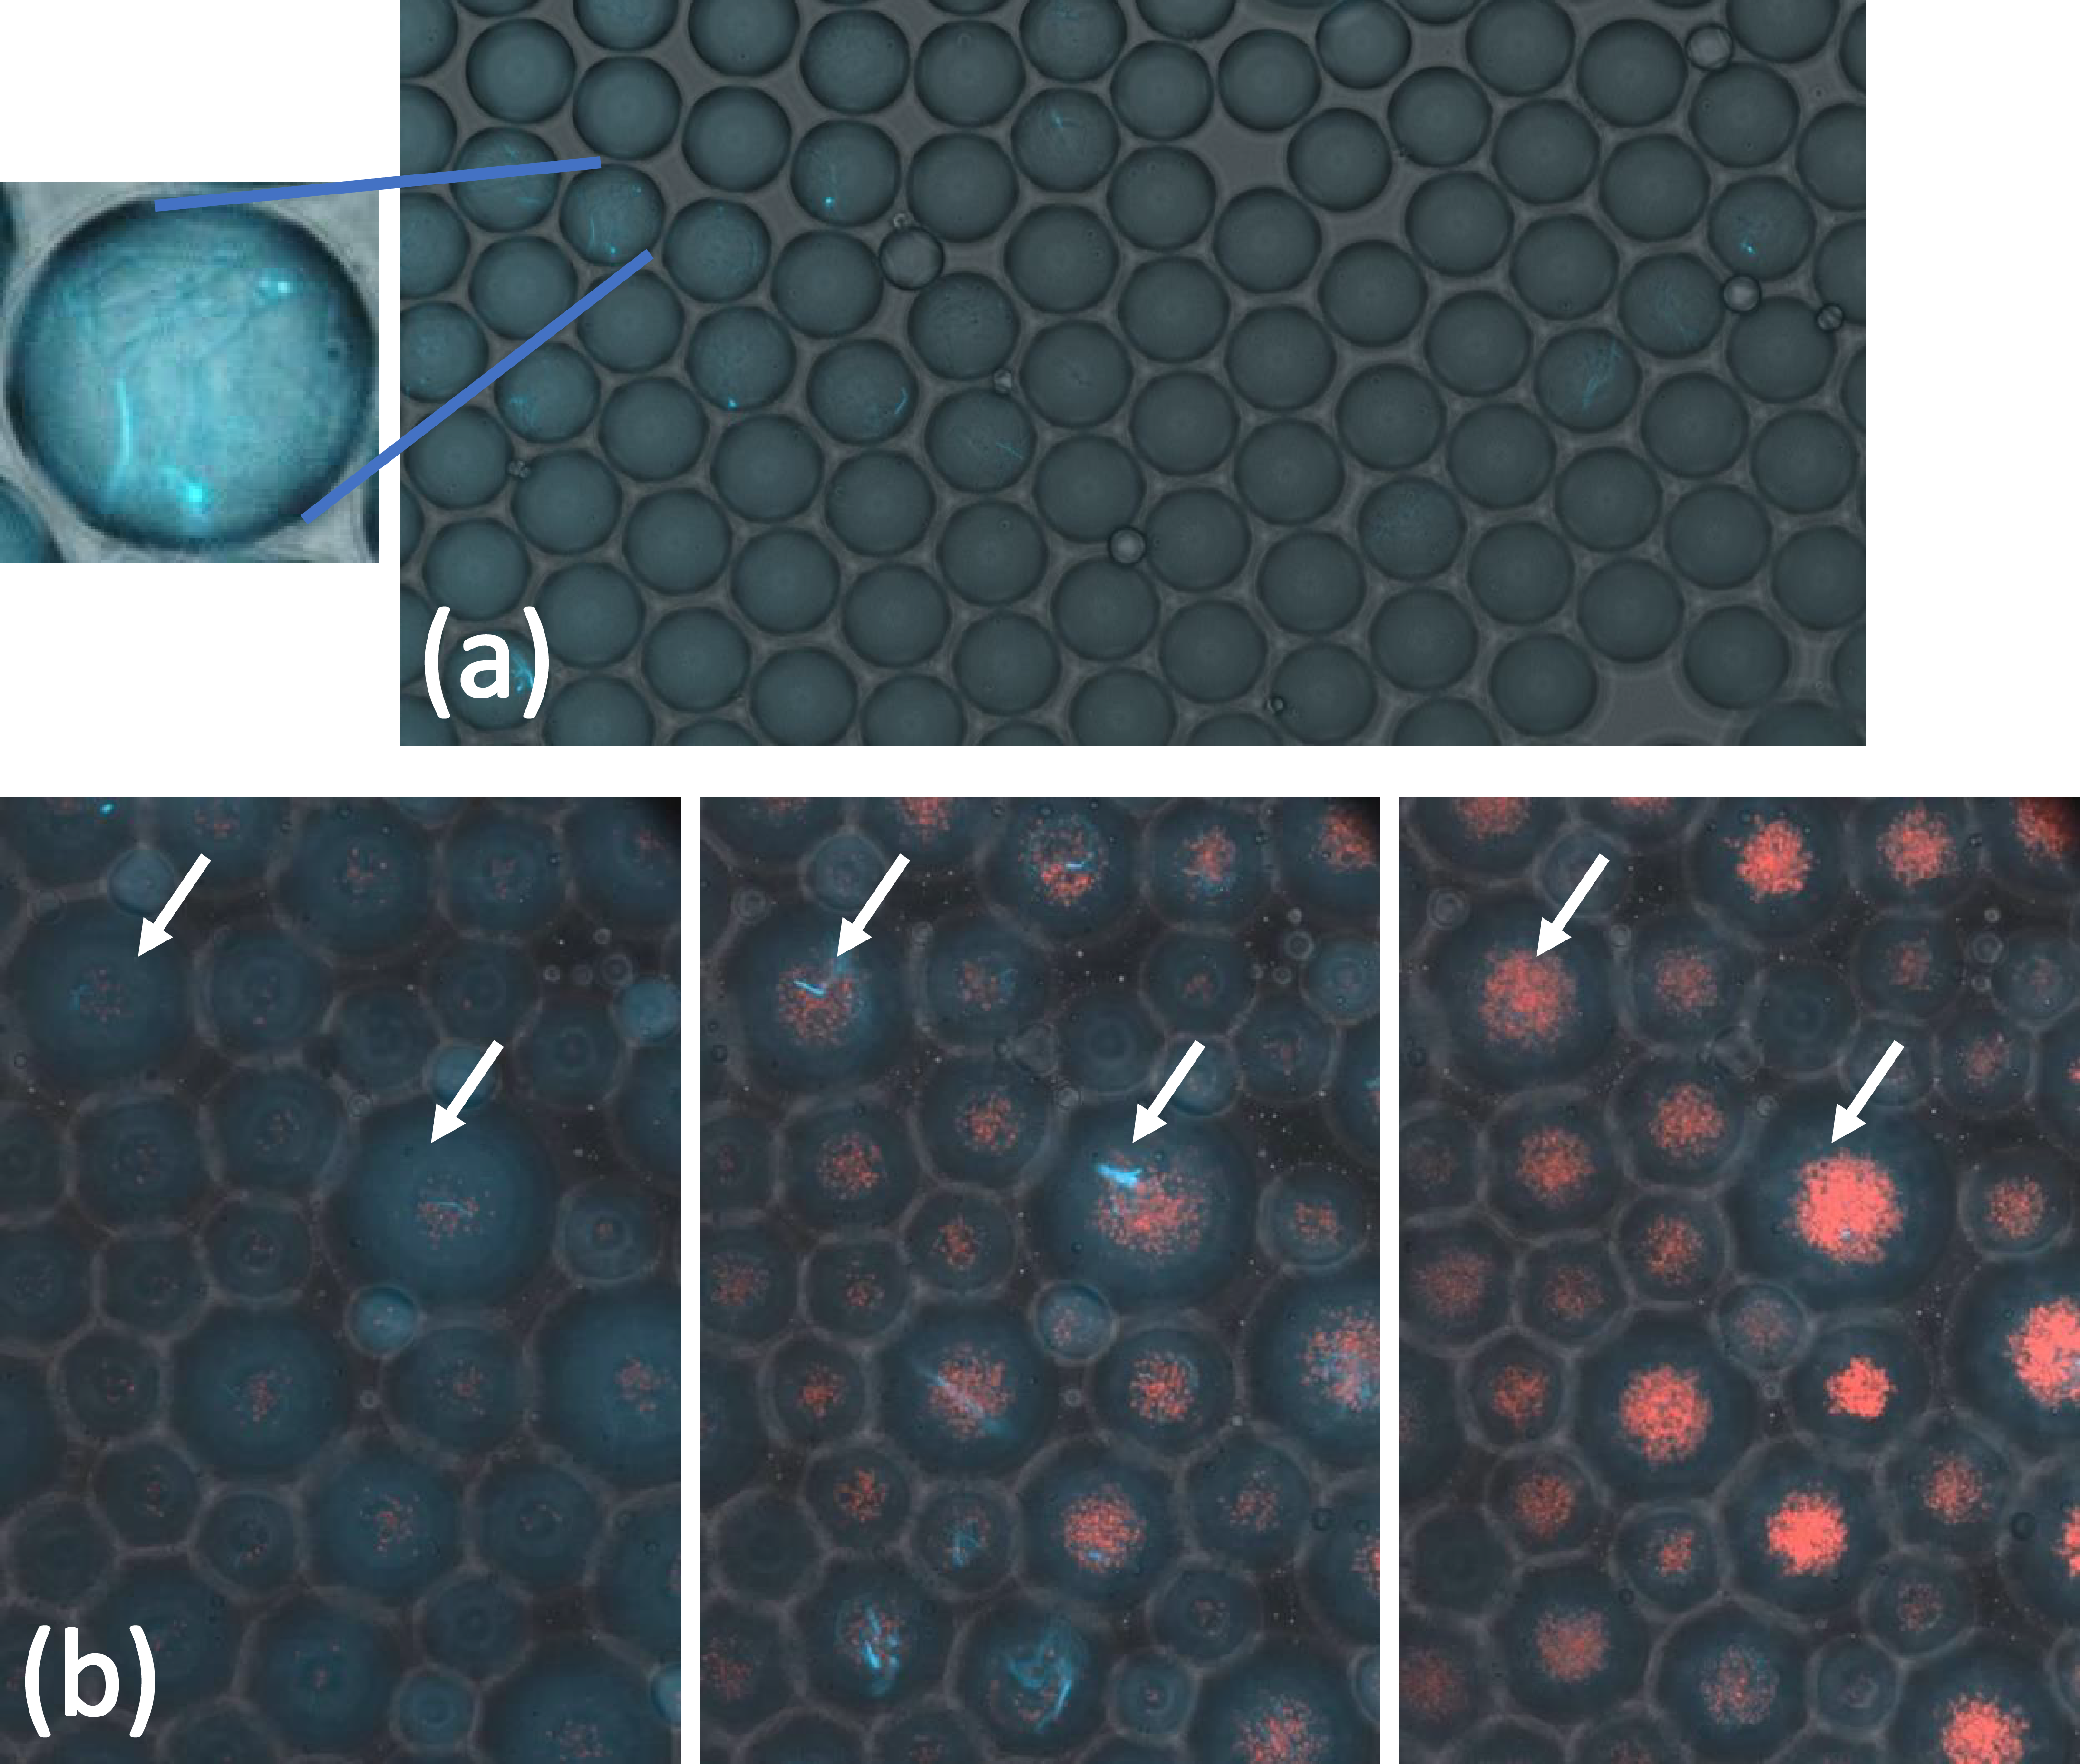
\includegraphics[width=\linewidth]{graphics/2025_09_30_droplets_fig8.png}
\caption{\textbf{On-chip droplets are stable after long-term incubation and allow bacterial growth} Our setup allows for long-term incubation and monitoring of droplets. (a) shows the results after 21h of incubation of droplets containing antibiotic producing bacteria alone in 30$^\circ$C without shaking. We observe stable same-sized droplets containing fluorescently tagged bacteria. The bacteria seem to be stressed and filament in the droplets. (b) shows snapshots of a time series of droplets containing both, antibiotic producing \textit{B. subtilis} (tagged in blue) and sensitive \textit{S. aureus} (tagged in red). Initially we see growth of both bacterial strains. However, \textit{B. subtilis} seems to be filamenting and at the end of the incubation, most droplets are filled exclusively with the target \textit{S. aureus} strain.}
\label{fig:results_incubation_subtilis}
\end{figure}
After establishing the technical platform, we can incubate droplets for long periods of time and can monitor them under the microscope during these incubation periods~(Figure~\ref{fig:results_incubation_subtilis}). Using the producer-target pair we selected, we encapsulate the producer alone~(after incubation in Figure~\ref{fig:results_incubation_subtilis}a) and together with the target strain (time series in Figure~\ref{fig:results_incubation_subtilis}b) in droplets. Encapsulating it alone, we observe long filaments of cells in the droplets after incubation. This indicates some kind of stress in this specific growth environment. When encapsulating it together with sensitive bacteria, we observe initial growth of both strains together~(Figure~\ref{fig:results_incubation_subtilis}b center) but we already see similar filaments like in the encapsulation alone. After a long incubation together we observe the absence of producers and dominance of the target strain. This might indicate that antibiotic producing bacteria are dying rather than killing sensitive bacteria in the droplets.

\section{Liquid vs. droplet comparison}
To understand if \textit{B. subtilis} disappears only in droplets or also in liquid, we performed a liquid-droplet comparison assay with separate cultures of \textit{B. subtilis} and \textit{S. aureus}. After incubation for 21h with high inoculation densities, we see that both liquid cultures exhibited growth while in droplets only the \textit{S. aureus} culture exhibits growth. The \textit{B. subtilis} culture in droplets seems to not grow during the incubation period but rather reduce in population size in the droplets~(Figure~\ref{fig:results_liquid_vs_drop_supernatant}a).

\begin{figure}
\centering
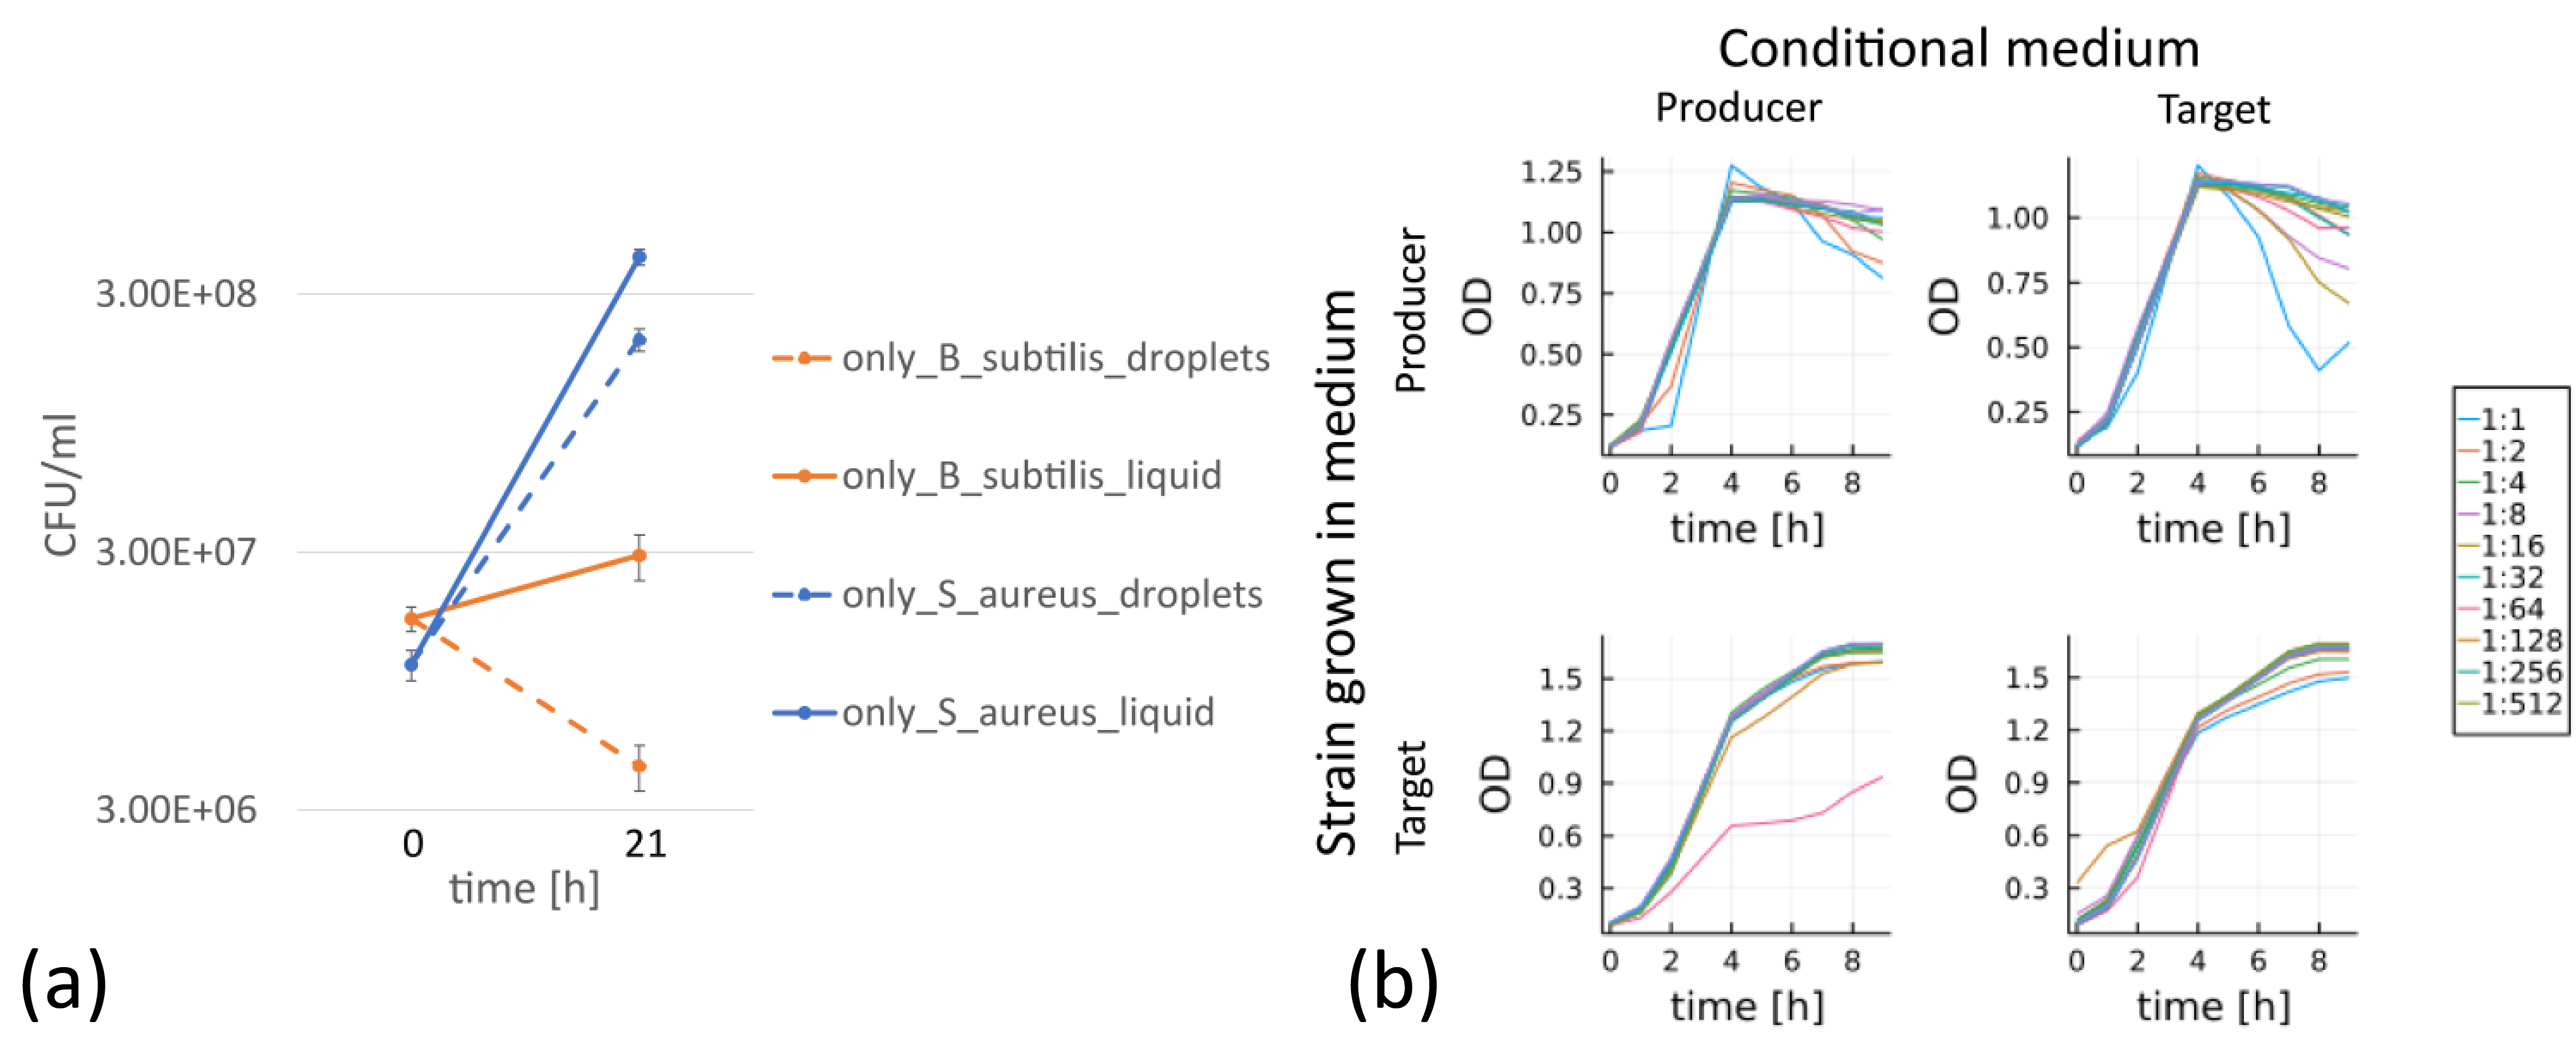
\includegraphics[width=\linewidth]{graphics/2025_09_30_droplets_fig9.png}
\caption{\textbf{\textit{B. subtilis} fails to grow in droplets and does not kill in liquid} To understand the observed dynamics in droplets, we conducted liquid experiments. (a) shows the results of comparing growth of antibiotic producing \textit{B. subtilis} in liquid and in droplets and similarly for the target \textit{S. aureus} strain. We observe that \textit{B. subtilis} seems to die in droplets while it grows in liquid culture. \textit{S. aureus} seems to grow almost equally well in droplets and liquid culture. (b) shows the results of growing bacteria in conditional medium. Studying every possible combination of producing and sensitive bacteria, we do not observe an effect of the antibiotic in liquid, hinting at the possible absence of toxic compounds in liquid compared to growth on solid media.}
\label{fig:results_liquid_vs_drop_supernatant}
\end{figure}

\section{Lack of antibiotic production in liquid}
To measure the efficiency of the produced compound, we use a conditional medium assay. We grow producer and target on its own or the other conditional medium respectively~(Figure~\ref{fig:results_liquid_vs_drop_supernatant})b). We do not measure a significant impact of the conditional medium on growth of bacteria in any of the conditions. Especially when growing the target strain on the conditional medium of the antibiotic producing strain. This indicates the lack of significant antibiotic production by the producer when grown in liquid, rendering it unusable in a droplet encapsulation scenario as it requires a liquid environment encapsulated in the droplet.